\documentclass[11pt,preprint, authoryear]{elsarticle}

\usepackage{lmodern}
%%%% My spacing
\usepackage{setspace}
\setstretch{1.2}
\DeclareMathSizes{12}{14}{10}{10}

% Wrap around which gives all figures included the [H] command, or places it "here". This can be tedious to code in Rmarkdown.
\usepackage{float}
\let\origfigure\figure
\let\endorigfigure\endfigure
\renewenvironment{figure}[1][2] {
    \expandafter\origfigure\expandafter[H]
} {
    \endorigfigure
}

\let\origtable\table
\let\endorigtable\endtable
\renewenvironment{table}[1][2] {
    \expandafter\origtable\expandafter[H]
} {
    \endorigtable
}


\usepackage{ifxetex,ifluatex}
\usepackage{fixltx2e} % provides \textsubscript
\ifnum 0\ifxetex 1\fi\ifluatex 1\fi=0 % if pdftex
  \usepackage[T1]{fontenc}
  \usepackage[utf8]{inputenc}
\else % if luatex or xelatex
  \ifxetex
    \usepackage{mathspec}
    \usepackage{xltxtra,xunicode}
  \else
    \usepackage{fontspec}
  \fi
  \defaultfontfeatures{Mapping=tex-text,Scale=MatchLowercase}
  \newcommand{\euro}{€}
\fi

\usepackage{amssymb, amsmath, amsthm, amsfonts}

\def\bibsection{\section*{References}} %%% Make "References" appear before bibliography


\usepackage[round]{natbib}

\usepackage{longtable}
\usepackage[margin=2.3cm,bottom=2cm,top=2.5cm, includefoot]{geometry}
\usepackage{fancyhdr}
\usepackage[bottom, hang, flushmargin]{footmisc}
\usepackage{graphicx}
\numberwithin{equation}{section}
\numberwithin{figure}{section}
\numberwithin{table}{section}
\setlength{\parindent}{0cm}
\setlength{\parskip}{1.3ex plus 0.5ex minus 0.3ex}
\usepackage{textcomp}
\renewcommand{\headrulewidth}{0.2pt}
\renewcommand{\footrulewidth}{0.3pt}

\usepackage{array}
\newcolumntype{x}[1]{>{\centering\arraybackslash\hspace{0pt}}p{#1}}

%%%%  Remove the "preprint submitted to" part. Don't worry about this either, it just looks better without it:
\makeatletter
\def\ps@pprintTitle{%
  \let\@oddhead\@empty
  \let\@evenhead\@empty
  \let\@oddfoot\@empty
  \let\@evenfoot\@oddfoot
}
\makeatother

 \def\tightlist{} % This allows for subbullets!

\usepackage{hyperref}
\hypersetup{breaklinks=true,
            bookmarks=true,
            colorlinks=true,
            citecolor=blue,
            urlcolor=blue,
            linkcolor=blue,
            pdfborder={0 0 0}}


% The following packages allow huxtable to work:
\usepackage{siunitx}
\usepackage{multirow}
\usepackage{hhline}
\usepackage{calc}
\usepackage{tabularx}
\usepackage{booktabs}
\usepackage{caption}


\newenvironment{columns}[1][]{}{}

\newenvironment{column}[1]{\begin{minipage}{#1}\ignorespaces}{%
\end{minipage}
\ifhmode\unskip\fi
\aftergroup\useignorespacesandallpars}

\def\useignorespacesandallpars#1\ignorespaces\fi{%
#1\fi\ignorespacesandallpars}

\makeatletter
\def\ignorespacesandallpars{%
  \@ifnextchar\par
    {\expandafter\ignorespacesandallpars\@gobble}%
    {}%
}
\makeatother

\newlength{\cslhangindent}
\setlength{\cslhangindent}{1.5em}
\newenvironment{CSLReferences}%
  {\setlength{\parindent}{0pt}%
  \everypar{\setlength{\hangindent}{\cslhangindent}}\ignorespaces}%
  {\par}


\urlstyle{same}  % don't use monospace font for urls
\setlength{\parindent}{0pt}
\setlength{\parskip}{6pt plus 2pt minus 1pt}
\setlength{\emergencystretch}{3em}  % prevent overfull lines
\setcounter{secnumdepth}{5}

%%% Use protect on footnotes to avoid problems with footnotes in titles
\let\rmarkdownfootnote\footnote%
\def\footnote{\protect\rmarkdownfootnote}
\IfFileExists{upquote.sty}{\usepackage{upquote}}{}

%%% Include extra packages specified by user

%%% Hard setting column skips for reports - this ensures greater consistency and control over the length settings in the document.
%% page layout
%% paragraphs
\setlength{\baselineskip}{12pt plus 0pt minus 0pt}
\setlength{\parskip}{12pt plus 0pt minus 0pt}
\setlength{\parindent}{0pt plus 0pt minus 0pt}
%% floats
\setlength{\floatsep}{12pt plus 0 pt minus 0pt}
\setlength{\textfloatsep}{20pt plus 0pt minus 0pt}
\setlength{\intextsep}{14pt plus 0pt minus 0pt}
\setlength{\dbltextfloatsep}{20pt plus 0pt minus 0pt}
\setlength{\dblfloatsep}{14pt plus 0pt minus 0pt}
%% maths
\setlength{\abovedisplayskip}{12pt plus 0pt minus 0pt}
\setlength{\belowdisplayskip}{12pt plus 0pt minus 0pt}
%% lists
\setlength{\topsep}{10pt plus 0pt minus 0pt}
\setlength{\partopsep}{3pt plus 0pt minus 0pt}
\setlength{\itemsep}{5pt plus 0pt minus 0pt}
\setlength{\labelsep}{8mm plus 0mm minus 0mm}
\setlength{\parsep}{\the\parskip}
\setlength{\listparindent}{\the\parindent}
%% verbatim
\setlength{\fboxsep}{5pt plus 0pt minus 0pt}



\begin{document}



\begin{frontmatter}  %

\title{Dynamic Portfolio Optimization Across Asset Classes using
Multi-variate Volatility Modelling}

% Set to FALSE if wanting to remove title (for submission)




\author[Add1]{Carel Olivier}
\ead{22017542@sun.ac.za}





\address[Add1]{22017542}



\vspace{1cm}


\begin{keyword}
\footnotesize{
Multivariate GARCH \sep DCC \sep Go-GARCH \sep Portfolio Optimization \\
\vspace{0.3cm}
}
\end{keyword}



\vspace{0.5cm}

\end{frontmatter}



%________________________
% Header and Footers
%%%%%%%%%%%%%%%%%%%%%%%%%%%%%%%%%
\pagestyle{fancy}
\chead{}
\rhead{}
\lfoot{}
\rfoot{\footnotesize Page \thepage}
\lhead{}
%\rfoot{\footnotesize Page \thepage } % "e.g. Page 2"
\cfoot{}

%\setlength\headheight{30pt}
%%%%%%%%%%%%%%%%%%%%%%%%%%%%%%%%%
%________________________

\headsep 35pt % So that header does not go over title




\hypertarget{introduction}{%
\section{\texorpdfstring{Introduction
\label{Introduction}}{Introduction }}\label{introduction}}

The idea of asset co-movements is important to investors because they
provide insight into the underlying relationships between assets and the
risk and return characteristics of a portfolio, which can inform
investment decisions and help to improve portfolio performance. In
particular, portfolio diversification helps to reduce the risk of large
losses by spreading investments across a variety of assets and can lead
to increased returns by providing exposure to a wider range of economic
and market conditions (\protect\hyperlink{ref-briere2012no}{Brière,
Chapelle \& Szafarz, 2012}).

A large body of literature has investigated the effect of the Global
Financial Crisis (GFC) on the relationship across various asset classes
(\protect\hyperlink{ref-mensi2016global}{Mensi, Hammoudeh, Nguyen \&
Kang, 2016}; \protect\hyperlink{ref-zhang2020global}{Zhang \&
Broadstock, 2020}). These studies have shown how the GFC has intensified
market relations and affected asset allocation and hedging strategies.
As such, fluctuations in interdependence across financial markets can
greatly affect investors seeking diversification benefits.

Several studies have examined the time-varying correlations between
asset classes in South Africa using various techniques. Bouri, Cepni,
Gabauer \& Gupta (\protect\hyperlink{ref-bouri2021return}{2021}), for
example, studied the dynamic connectedness across five assets using the
TVP-VAR connectedness approach. Bouri \emph{et al.}
(\protect\hyperlink{ref-bouri2021return}{2021}) shows that total
connectedness spiked around the COVID-19 outbreak, which subsequently
altered the structure of the network of connectedness and posed a threat
to investors' portfolios. Horvath \& Poldauf
(\protect\hyperlink{ref-horvath2012international}{2012}) studied the
conditional correlation between sectors of numerous economies, including
South Africa, using the BEKK MV-GARCH approach. Duncan \& Kabundi
(\protect\hyperlink{ref-duncan2013domestic}{2013}) used generalised
variance decompositions of a vector autoregressive model to study the
time-varying domestic and foreign volatility spillovers and evolving
linkages across asset classes in South Africa and global capital
markets.

The analysis in this paper is divided into two parts. First, I will
analyse the time-varying conditional correlations between the different
asset classes by using Engle
(\protect\hyperlink{ref-engle2002dynamic}{2002}) Dynamic Conditional
Correlation (DCC) Model as well as a GO-GARCH model. DCC models are
statistical models used in finance and economics to capture the changing
correlations between multiple time series. These models allow for
changes in the correlations between time series over time, which is
important in modelling the behaviour of assets that are dependent on
each other (\protect\hyperlink{ref-engle2002dynamic}{Engle, 2002}). DCC
models use a multivariate GARCH framework to capture the dynamics of the
covariance matrix of the series over time.

The second part of the analysis will focus on portfolio optimization.
Portfolio optimization is the process of determining the optimal
allocation of assets in a portfolio in order to maximize returns or
minimize risk. This typically involves using mathematical models to
identify the portfolio that offers the best trade-off between risk and
return, taking into account constraints such as investment budgets and
risk tolerance (\protect\hyperlink{ref-ledoit2003improved}{Ledoit \&
Wolf, 2003}). The optimization process takes into account factors such
as expected returns, volatilities, and correlations between assets in
order to determine the optimal portfolio mix.

\hypertarget{methodology}{%
\section{Methodology}\label{methodology}}

\hypertarget{dcc-specification}{%
\subsection{DCC specification}\label{dcc-specification}}

The method behind DCC models is based on the idea of modeling the
covariance matrix of the returns of multiple assets over time. For Engle
(\protect\hyperlink{ref-engle2002dynamic}{2002}) DCC model the
variance-covariance matrix can be written as \footnote{The paper was
  written using the `Texevier' package developed by N.F. Katzke (2016)}:

\begin{equation} \label{dcc}
H_t = D_t.R_t.D_t.
\end{equation}

Estimating \(R_T\) now requires it to be inverted at each estimated
period, and thus a proxy equation is used:

\begin{align}  \label{dcc2}
  Q_{ij,t} &= \bar Q + a\left(z_{t - 1}z'_{t - 1} - \bar{Q} \right) + b\left( Q_{ij, t - 1} - \bar{Q} \right) \hfill \\ \notag
        &= (1 - a - b)\bar{Q} + az_{t - 1}z'_{t - 1} + b.Q_{ij, t - 1} \notag
\end{align}

With non-negative scalars \(a\) and \(b\), and with:

\begin{itemize}
\item
  \(Q_{ij, t}\) the unconditional (sample) variance estimate between
  series \(i\) and \(j\) ,
\item
  \(\bar{Q}\) the unconditional matrix of standardized residuals from
  each univariate pair estimate.
\end{itemize}

We next estimate \(R_T\) as:

\begin{align}\label{eq:dcc3}
R_t &= diag(Q_t)^{-1/2}Q_t.diag(Q_t)^{-1/2}. 
\end{align}

The dynamic conditional correlation matrix, will therefore have entries
in the bivariate framework as follows:

\begin{align}
R_t &= \rho_{ij,t} = \frac{q_{i,j,t}}{\sqrt{q_{ii,t}.q_{jj,t}}} 
\end{align}

\hypertarget{go-garch-specification}{%
\subsection{Go-GARCH specification}\label{go-garch-specification}}

The methodology behind Go-GARCH models is based on a combination of the
GARCH (Generalized Autoregressive Conditional Heteroskedasticity)
framework and the concept of orthogonalization. Orthogonalization is
used to ensure that the parameters of the model are estimated in an
uncorrelated and unbiased manner. This can help to improve the stability
and accuracy of the model's predictions.

These orthogonal components are measured by identifying independent and
uncorrelated factors that make up the var-covar matrix \(H_t\). The
statistical transformations are done as follows:

\begin{align}
r_t &= \mu_t +\varepsilon_t  \\
\varepsilon_t &= A.f_t 
\end{align}

with \(A\) linking the unobserved uncorrelated components with the
observed residual process. Also: \(f_t\) represents the unobserved
independent factors assigned to each series (factor weights), such that:

\begin{align}
    f_t = H^{1/2}.z_t
\end{align}

with \(H_T\) and \(z_t\) as before and:

\begin{align}
E[f_t] &= 0 ; \qquad \qquad E[f_tf_t'] = I_N \notag \\
E[\varepsilon_t] &= 0 ; \qquad \qquad E[\varepsilon_t\varepsilon_t'] = AA'
\end{align}

So that the conditional covariance matrix is given by:

\begin{align}
    \Sigma_t=AH_tA'
\end{align}

\hypertarget{data}{%
\section{Data}\label{data}}

My objective is to characterise the time-varying correlation estimates
to provide insight into the underlying comovement structures of a
portfolio of asset classes. The empirical application in this paper aims
to diversify a portfolio investing in stocks, property, gold, and
Bitcoin. This study collects daily price data on the FTSE/JSE Africa All
Share Index, FTSE/JSE Africa Property Index, gold, and Bitcoin
\footnote{All the data was obtained from the `fmxdat' package in R}. The
sample period of this study covers data from the beginning of 2015 to
the end of 2019. Considering a time series of prices, the daily asset
returns are calculated by taking the log difference of each index
series, as:

\begin{align} 
  r_{i,t} &= ln(\frac{P_{i,t}}{P_{i,t-1}}) * 100
\end{align}

Where \(P_{i,t}\) is the closing price of the index, \(i\), at time
\(t\). Logarithmic returns are usually preferred by financial
econometricians because of their superior properties compared to
arithmetic returns.

In order to analyse the characteristics of the data for the return
series, I first produce a chart of the price and return series. The two
figures below shows the closing prices and returns of the four asset
classes, respectively. We can see from the second figure that the return
series exhibit volatility clustering.

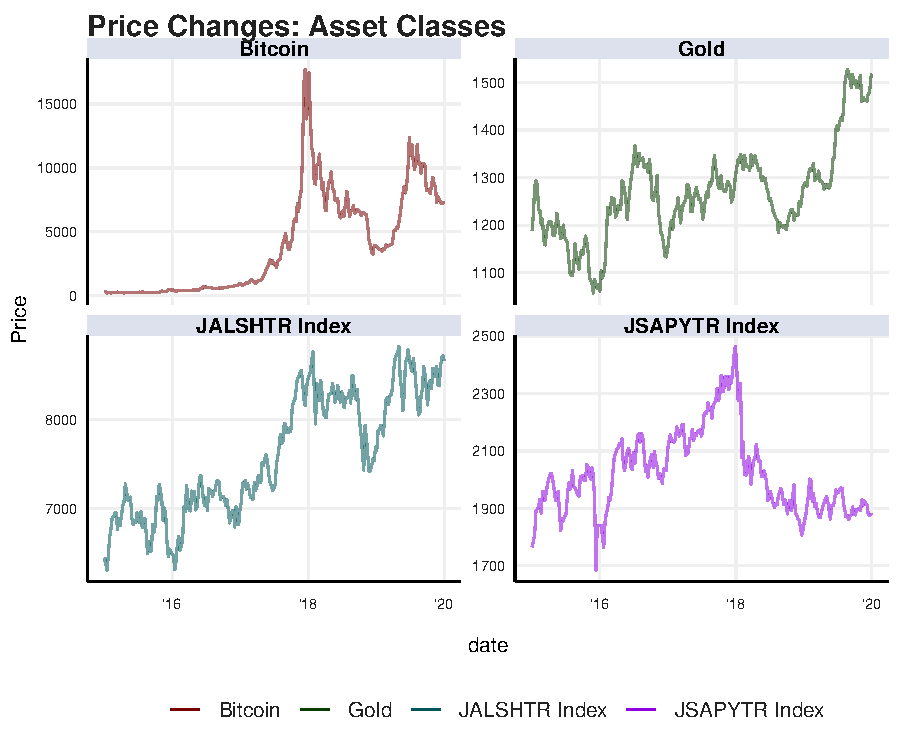
\includegraphics{FinMetrics-Essay_files/figure-latex/unnamed-chunk-1-1.pdf}

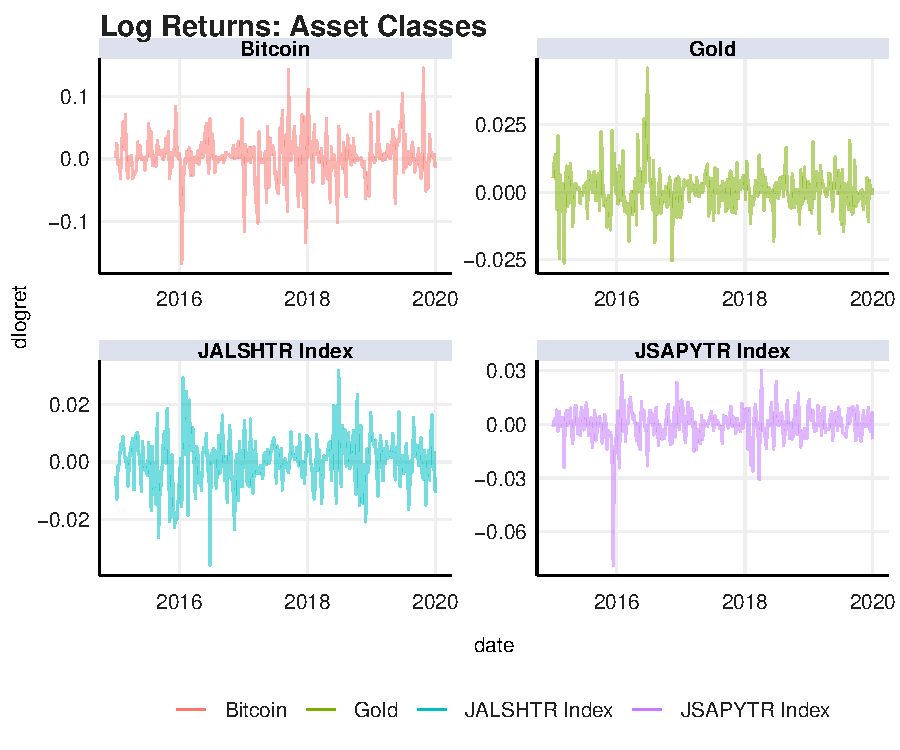
\includegraphics{FinMetrics-Essay_files/figure-latex/unnamed-chunk-2-1.pdf}

Next, I examine the Autoregressive Conditional Heteroskedasticity (ARCH)
effects. To visualize the analysis of autocorrelations in the residuals
and squared residuals, I graph the returns, squared returns and the
absolute returns for an equally weighted portfolio of the assets using
simple returns.

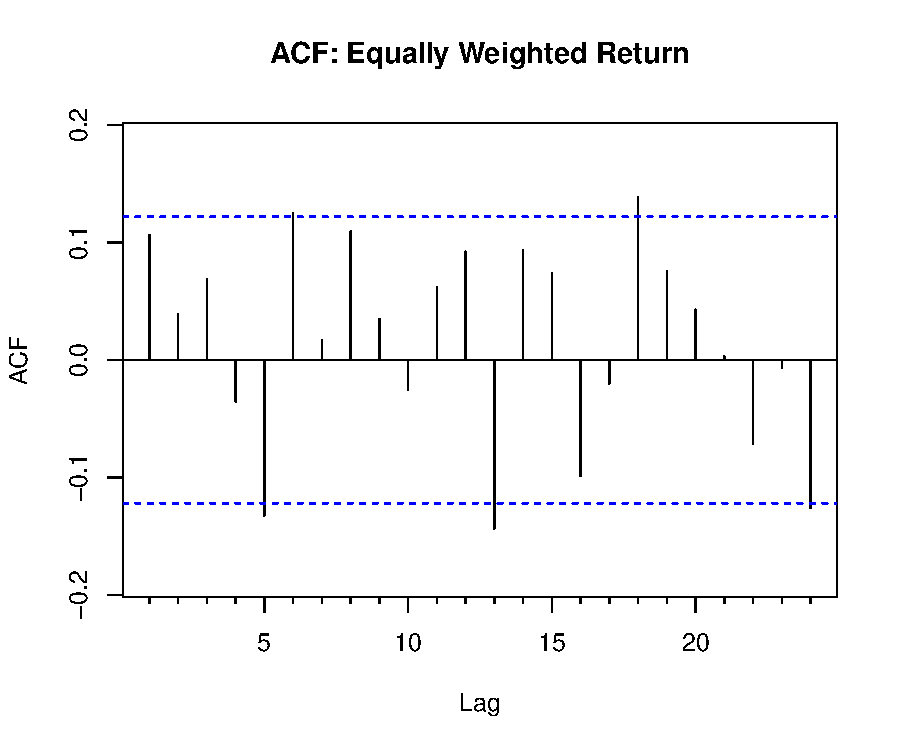
\includegraphics{FinMetrics-Essay_files/figure-latex/unnamed-chunk-4-1.pdf}

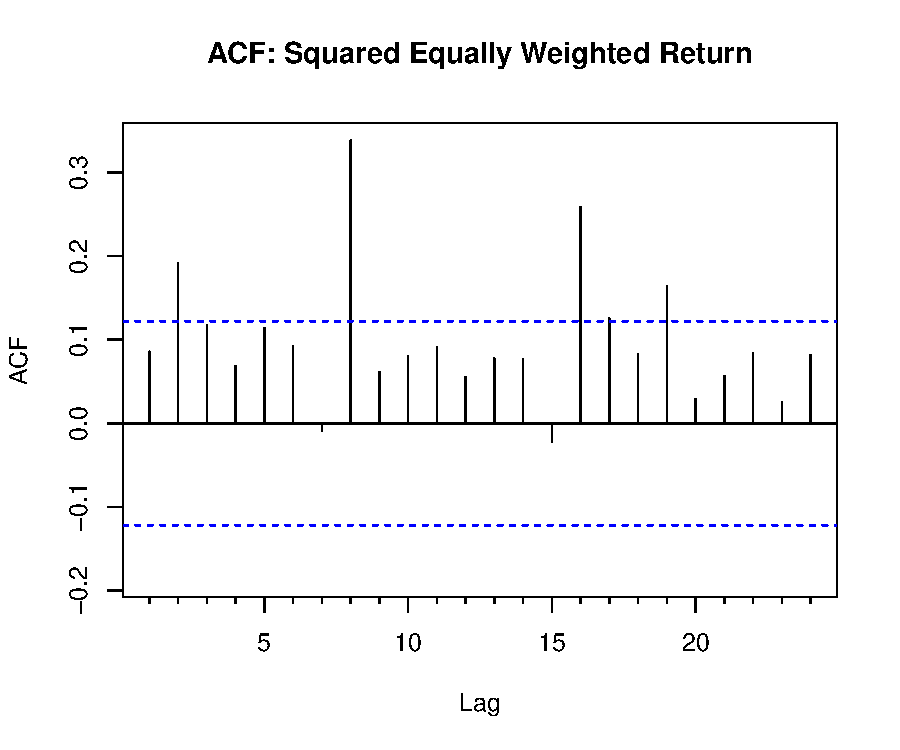
\includegraphics{FinMetrics-Essay_files/figure-latex/unnamed-chunk-5-1.pdf}

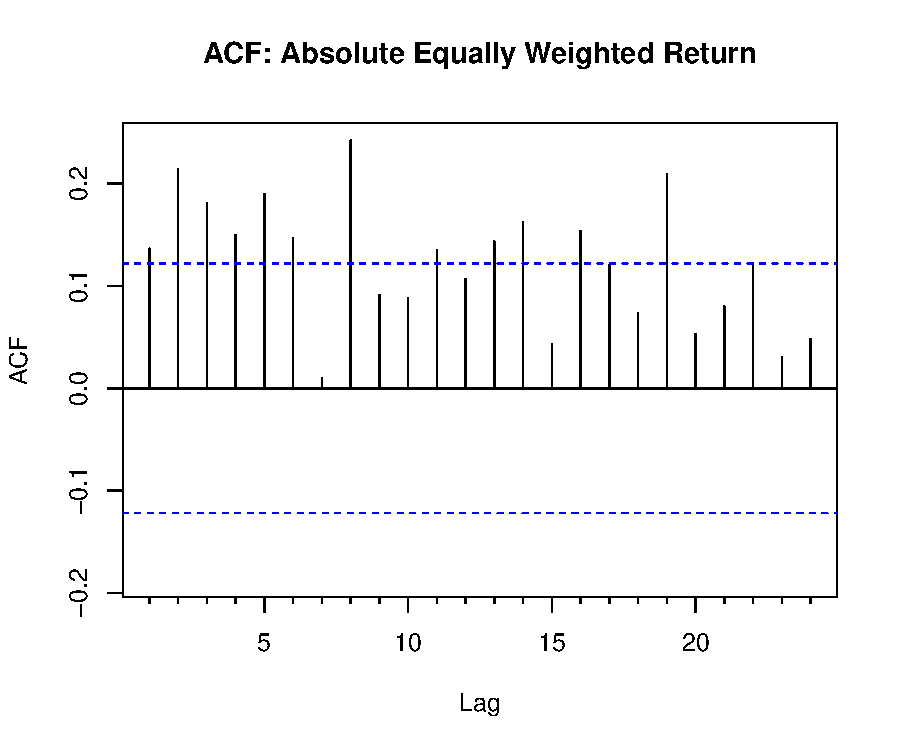
\includegraphics{FinMetrics-Essay_files/figure-latex/unnamed-chunk-6-1.pdf}

The above figure displays a pattern of squared residuals, which
indicates strong conditional heteroskedasticity. In addition, I formally
test for ARCH effects using a Ljung--Box test which rejected the null of
no ARCH effects - hence I need to control for the remaining conditional
heteroskedasticity in the returns series.

\hypertarget{dcc-model}{%
\section{DCC model}\label{dcc-model}}

Before fitting the most appropriate univariate GARCH specifications to
each series, I check and clean the data for any missing values and
outliers. Thereafter, I specify a GARCH model for each time series,
which is used as the conditional covariance structure in the DCC model.
Finally, I compute the dynamic correlations between each pair of assets.

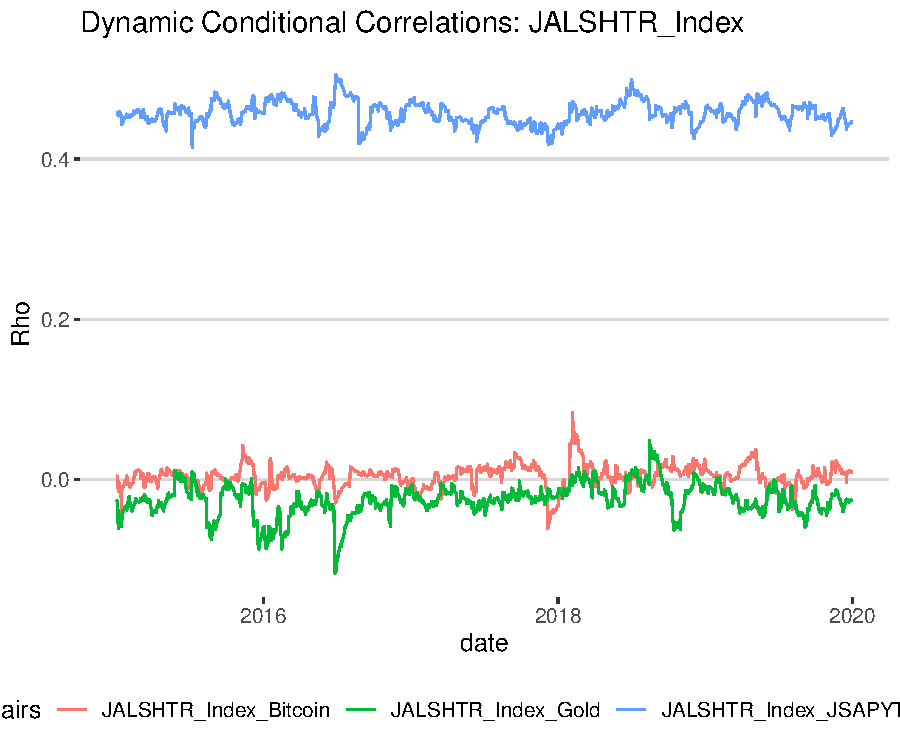
\includegraphics{FinMetrics-Essay_files/figure-latex/unnamed-chunk-8-1.pdf}

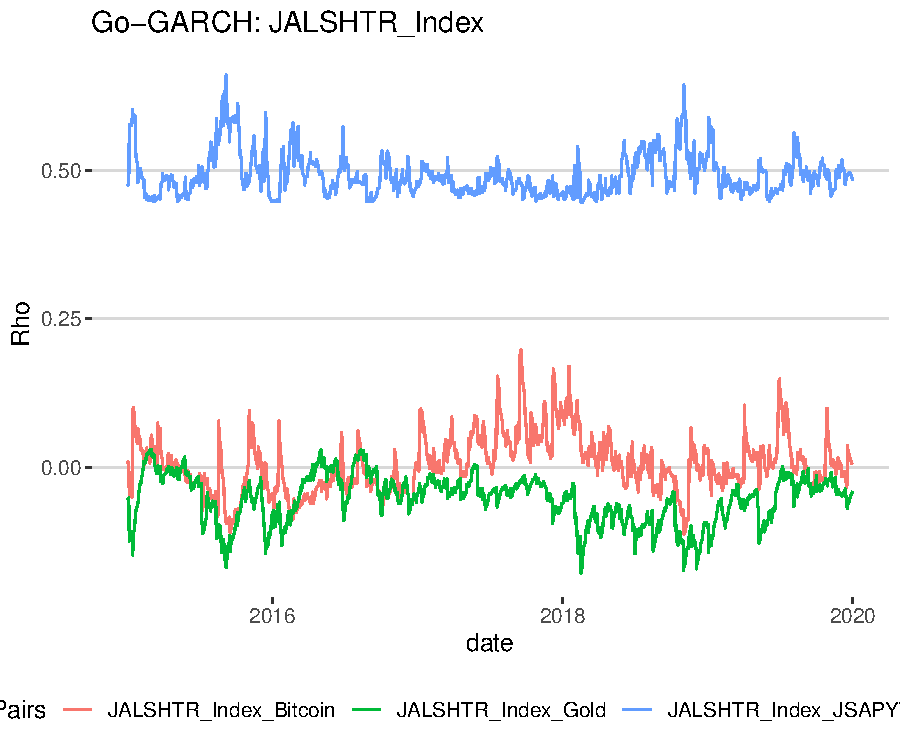
\includegraphics{FinMetrics-Essay_files/figure-latex/unnamed-chunk-9-1.pdf}

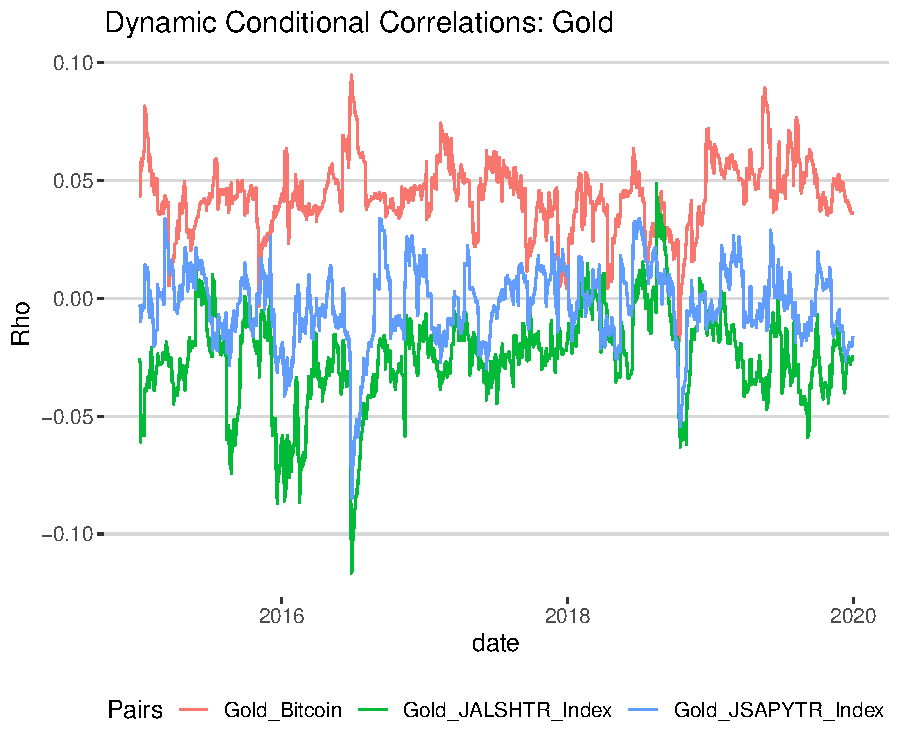
\includegraphics{FinMetrics-Essay_files/figure-latex/unnamed-chunk-10-1.pdf}

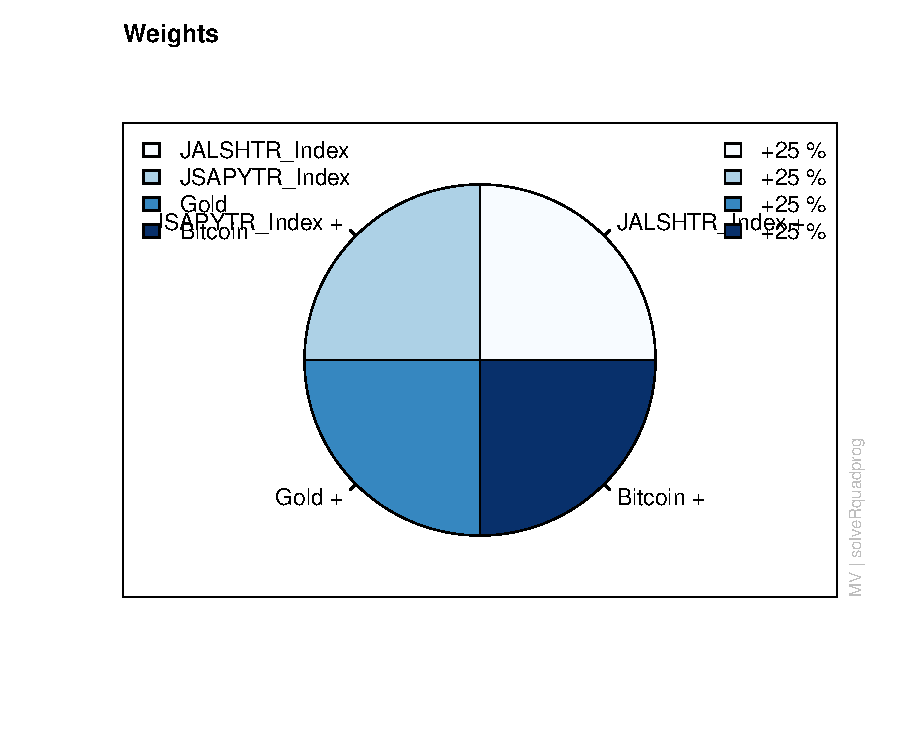
\includegraphics{FinMetrics-Essay_files/figure-latex/unnamed-chunk-11-1.pdf}

The figures above illustrate the evolution of correlation processes over
time. Some asset pairs show correlations that are very volatile and some
that flow from positive to negative, or from negative to positive. It
indicates that the diversification potential changes over time.

\hypertarget{go-garch}{%
\section{Go-GARCH}\label{go-garch}}

Generalized Orthogonal GARCH (GO-GARCH) models are used to model and
forecast volatility in financial time series data. GO-GARCH models are
an extension of the popular GARCH (Generalized Autoregressive
Conditional Heteroskedasticity) models and combine features of both ARCH
(Autoregressive Conditional Heteroskedasticity) and GARCH models.
GO-GARCH models are characterized by using orthogonal (uncorrelated)
innovations in the GARCH process, which results in a reduced number of
parameters compared to traditional GARCH models
(\protect\hyperlink{ref-boswijk2006wake}{Boswijk \& Weide, 2006}). This
makes the GO-GARCH models computationally more efficient and easier to
estimate. Additionally, the use of orthogonal innovations can lead to
better forecasting performance, especially in situations where the
underlying volatility process is highly non-linear.

The figure below depict the time-varying correlations between the asset
classes using a GO-GARCH model.

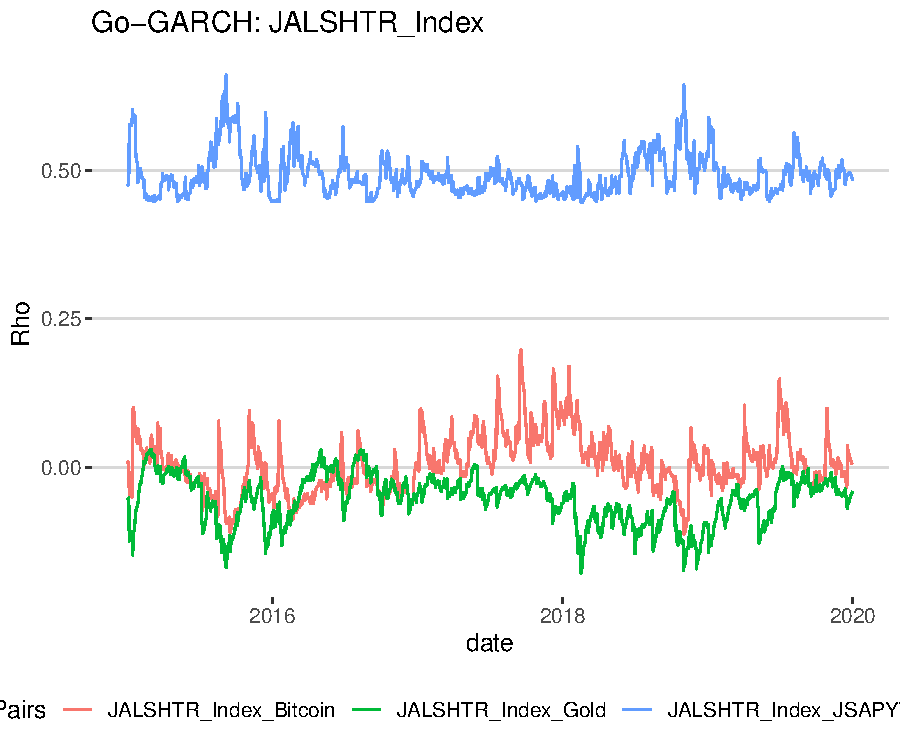
\includegraphics{FinMetrics-Essay_files/figure-latex/unnamed-chunk-14-1.pdf}

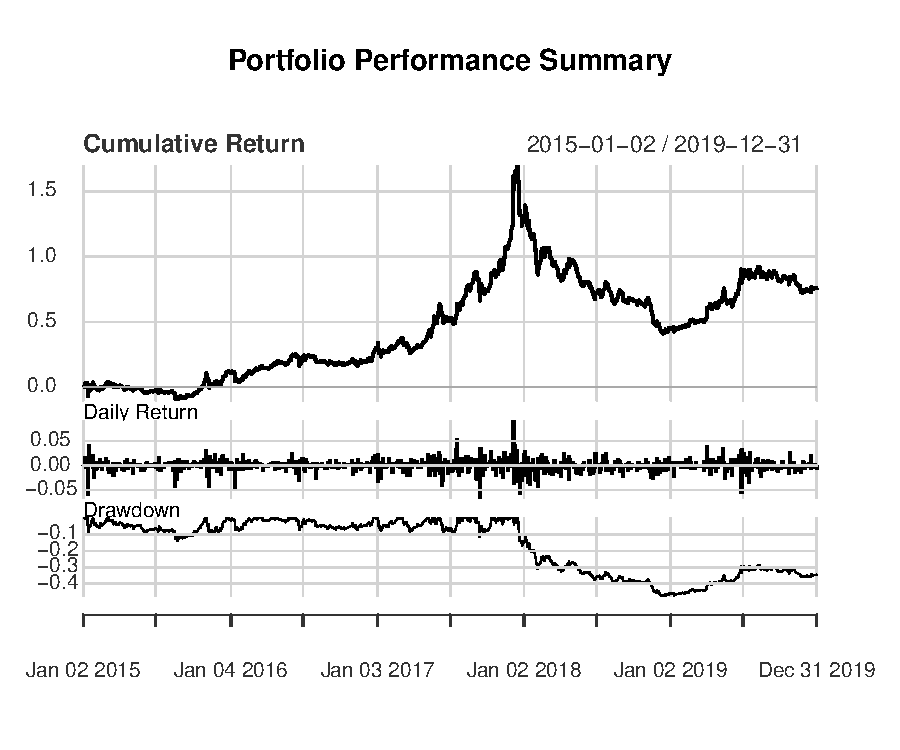
\includegraphics{FinMetrics-Essay_files/figure-latex/unnamed-chunk-15-1.pdf}

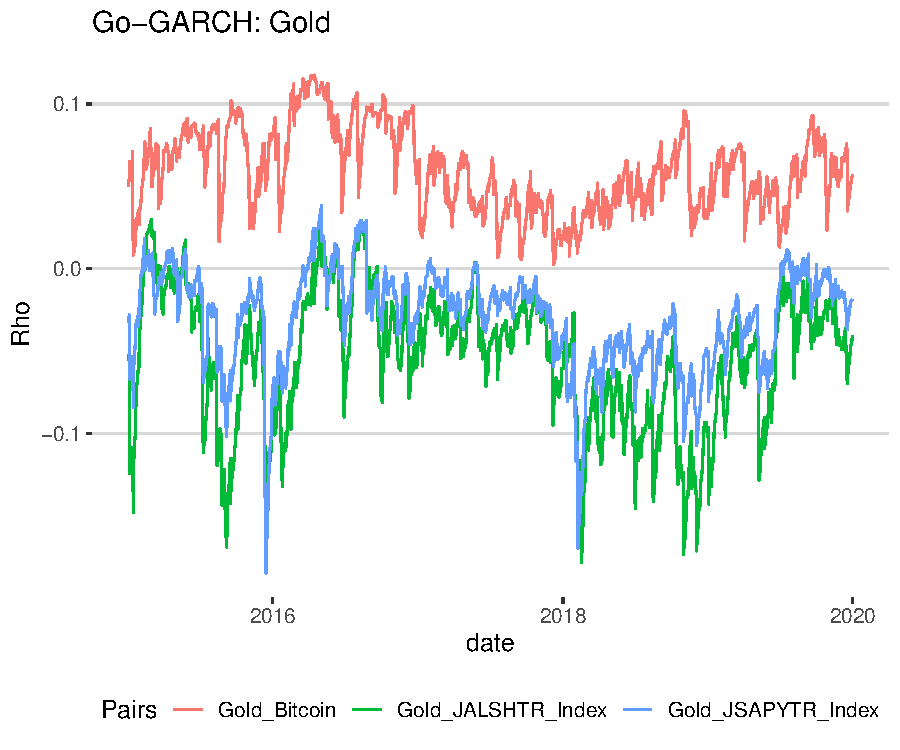
\includegraphics{FinMetrics-Essay_files/figure-latex/unnamed-chunk-16-1.pdf}

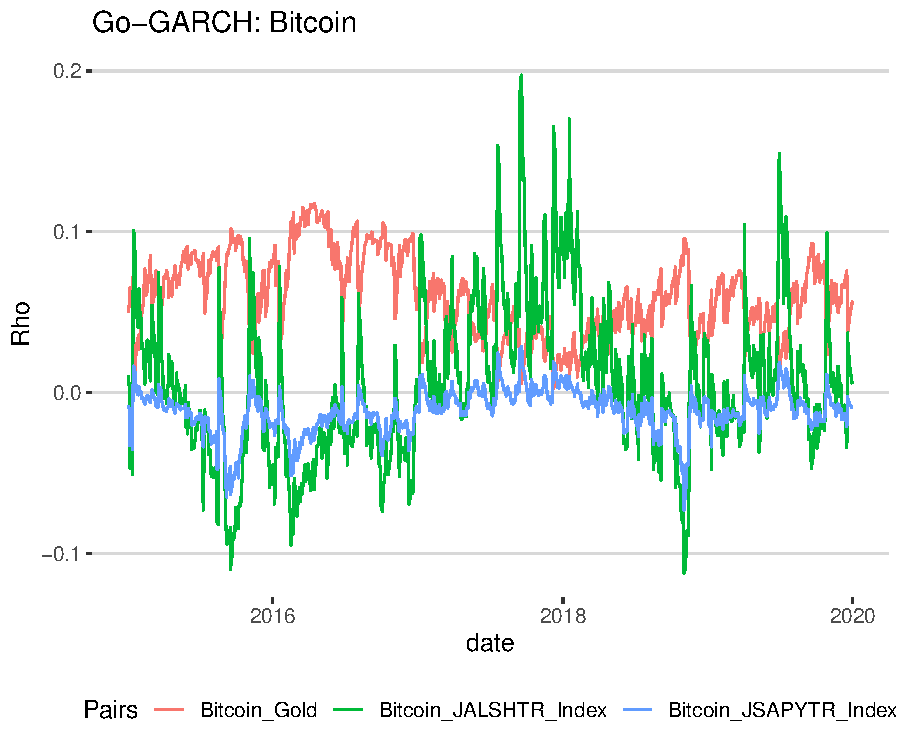
\includegraphics{FinMetrics-Essay_files/figure-latex/unnamed-chunk-17-1.pdf}

The most noticeable difference between the GO-GARCH correlations and the
DCC correlations is the range in which they vary. Similar to Boswijk \&
Weide (\protect\hyperlink{ref-boswijk2006wake}{2006}) I find that the
GO-GARCH and DCC correlation patterns are similar, however, from my
analyse I do not find that the GO-GARCH model behaves like a smoothed
version of the DCC model. Furthermore, the difference between these two
models should be interpreted with caution since this property may be
favourable to some and not others.

\hypertarget{portfolio-optimization}{%
\section{Portfolio optimization}\label{portfolio-optimization}}

In the final section of this paper, I use the data on equities,
property, gold and Bitcoin to optimize three portfolios with a linear
constraint of long only. In particular, I construct an equal weight
portfolio, a global minimum variance portfolio, and a tangency
portfolio. The equal weight portfolio gives equal weights of 25 percent
to each of the assets in the portfolio. The global minimum portfolio
refers to a portfolio that has the minimum possible risk or variance
among all possible portfolios constructed from the set of assets. In
other words, it is the portfolio with the lowest possible risk among all
portfolios with a given expected return. Finally, the tangency portfolio
is a portfolio that lies on the efficient frontier and is the portfolio
with the highest Sharpe ratio. The Sharpe ratio is a measure of the
risk-adjusted return of an investment, defined as the excess return over
the risk-free rate divided by the standard deviation of the investment's
returns (\protect\hyperlink{ref-sharpe1966mutual}{Sharpe, 1966}).

The pie charts below illustrate the optimal weighting as defined by the
equally weighted, global minimum, and tangency portfolios',
respectively. As expected, we see that Bitcoin receives a very small
weighting (1.3\%) in the global minimum portfolio since it is deemed
high risk.

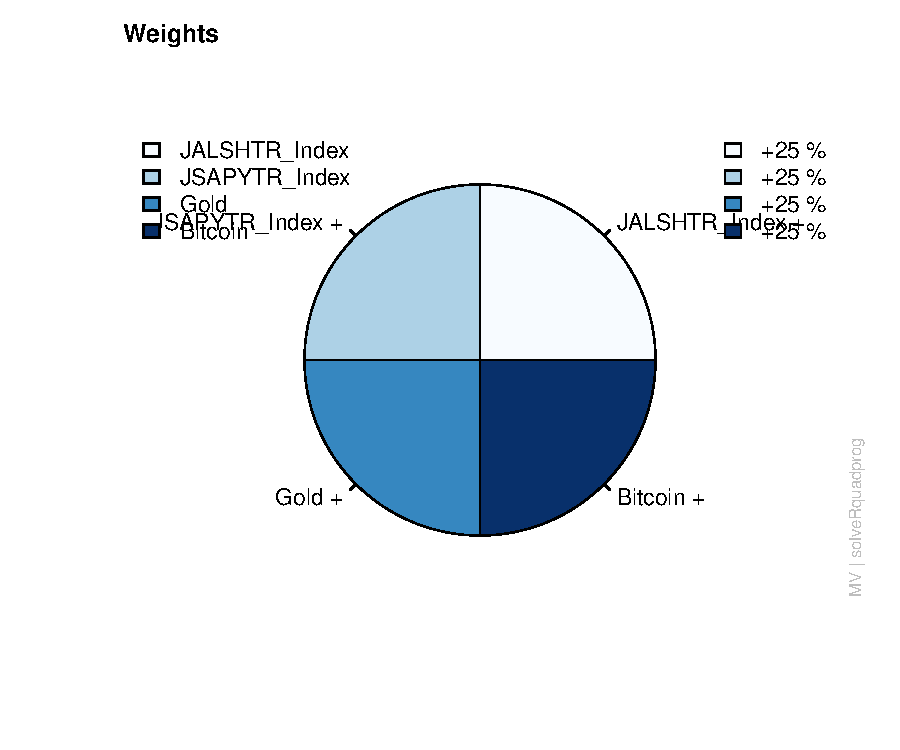
\includegraphics{FinMetrics-Essay_files/figure-latex/unnamed-chunk-20-1.pdf}

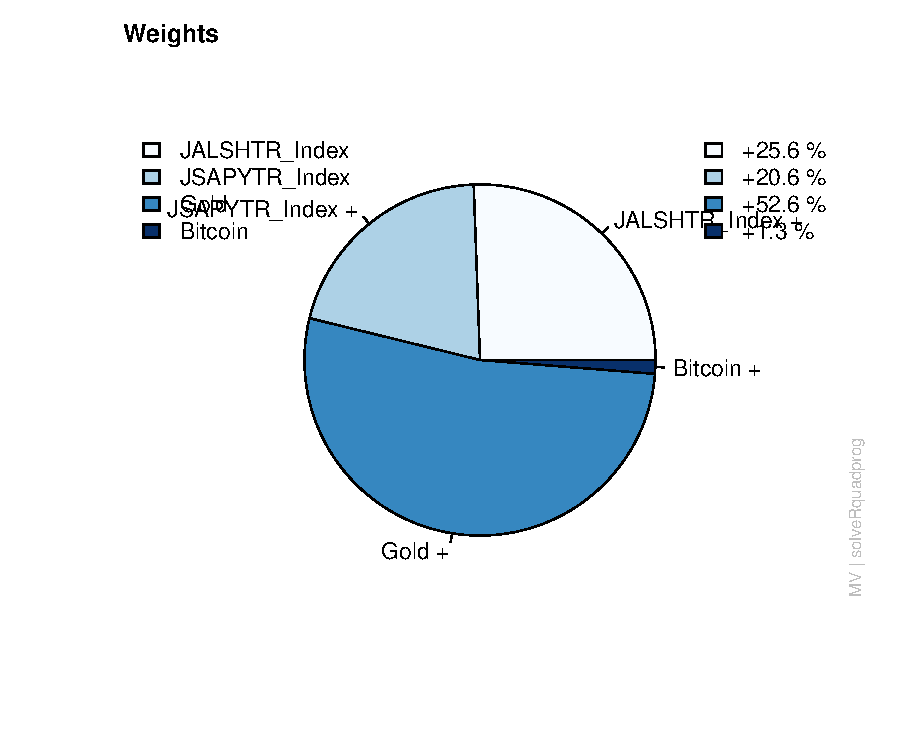
\includegraphics{FinMetrics-Essay_files/figure-latex/unnamed-chunk-21-1.pdf}

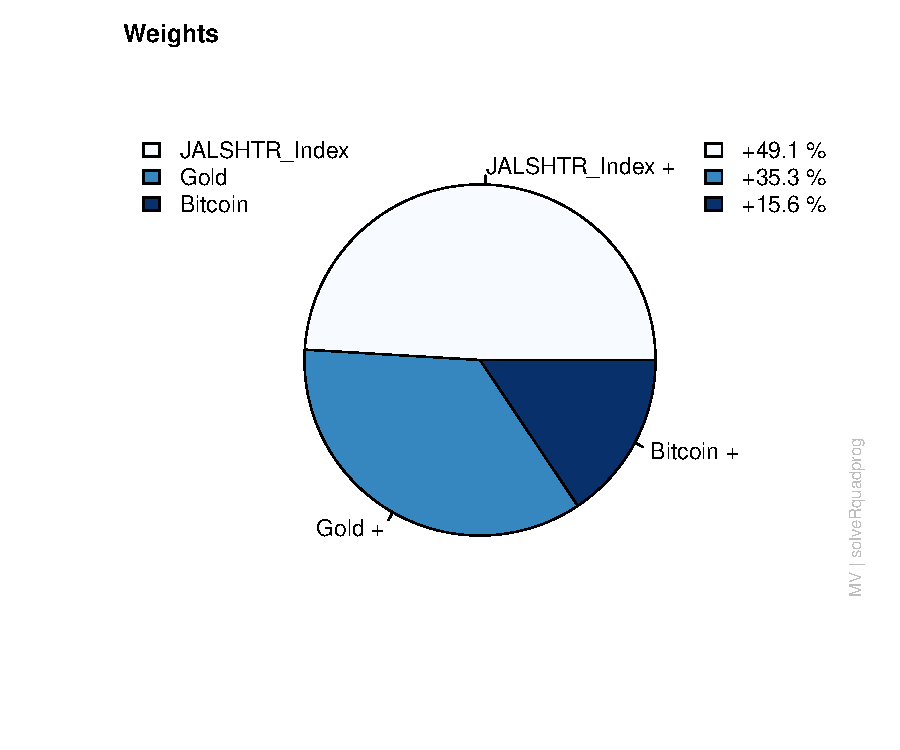
\includegraphics{FinMetrics-Essay_files/figure-latex/unnamed-chunk-22-1.pdf}

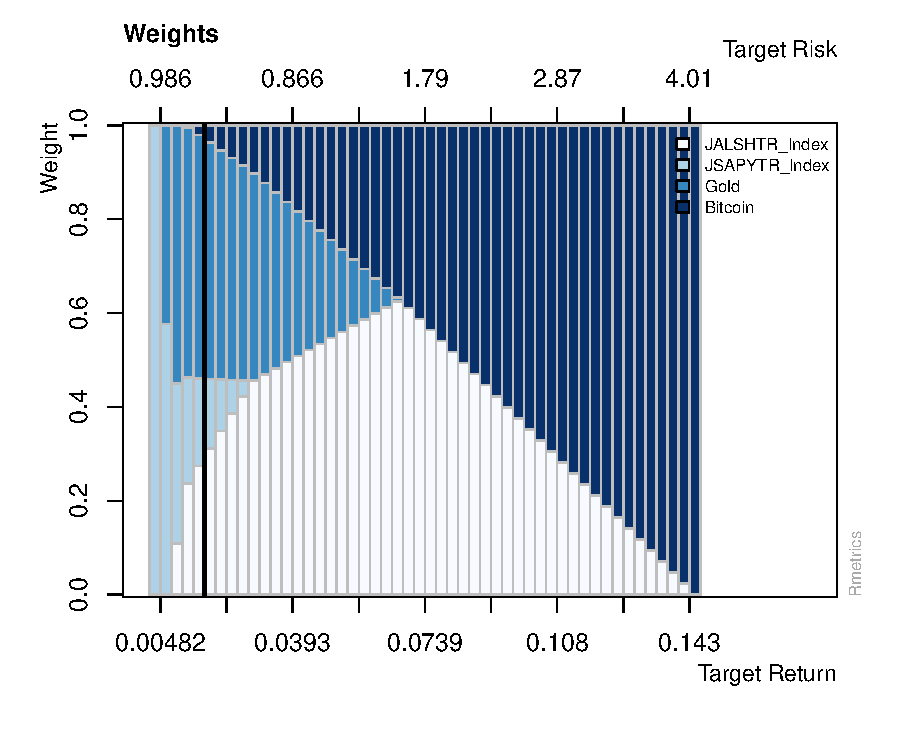
\includegraphics{FinMetrics-Essay_files/figure-latex/unnamed-chunk-23-1.pdf}

The figure above is another interesting chart that displays the weights
on the different assets, the risk, and the return along the frontier.
The black line through the chart indicates the minimum variance
portfolio.

Next, I present the performance summary charts which sums up the
information we need in analysing all the portfolios' performance over
time. The charts depict each portfolio's cumulative return, daily
return, and drawdown. Each portfolio is rebalanced every quarter.

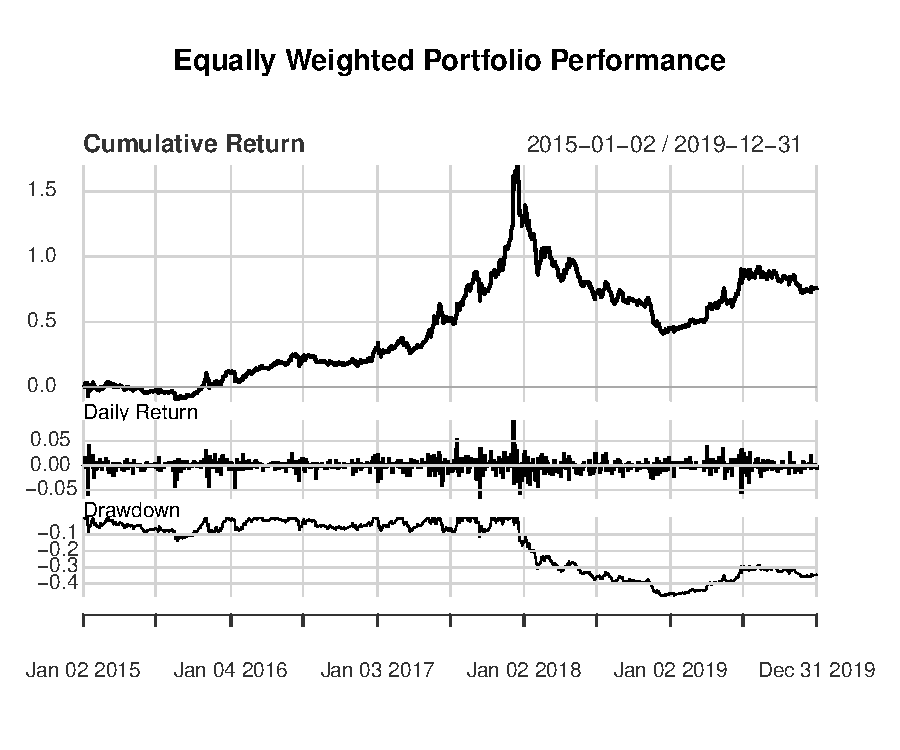
\includegraphics{FinMetrics-Essay_files/figure-latex/unnamed-chunk-25-1.pdf}

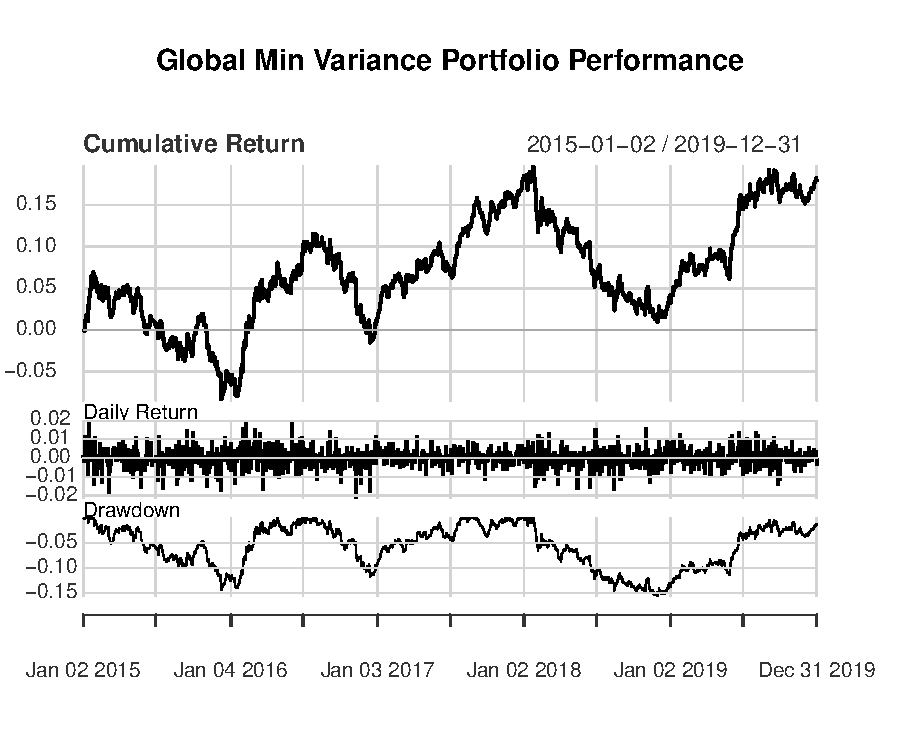
\includegraphics{FinMetrics-Essay_files/figure-latex/unnamed-chunk-27-1.pdf}

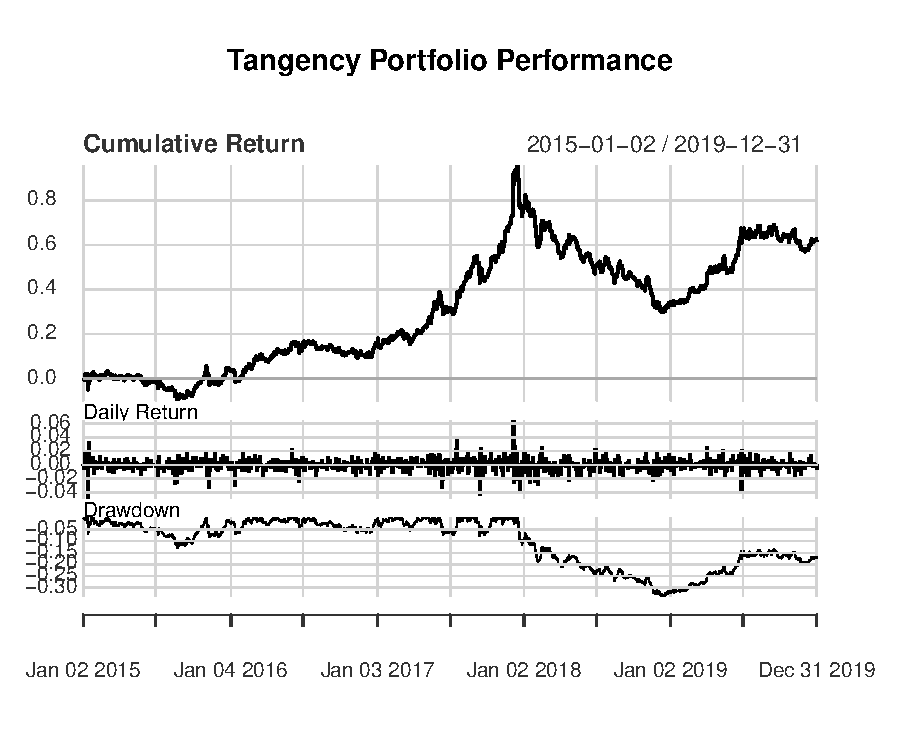
\includegraphics{FinMetrics-Essay_files/figure-latex/unnamed-chunk-29-1.pdf}

Finally, the table displays the target returns and risks associated with
each portfolio.

\[
\begin{array}{|c|c|c|c|c|}
\hline \text { Portfolio } & \text { Mean Return } & \text { Cov } & \text { CVaR } & \text { VaR }  \\
\hline \text { Equally Weighted } & { 0.0464 } & {1.1288 } & {2.7860 } & {1.8735 }\\
\text { Global Minimum Variance } & {0.0149 } & {0.5473 } & {1.2432} & {0.9095 } \\
\text { Tangency } & {0.0383 } & {0.8425 } & {1.9634 } & {1.3444 } \\
\hline
\end{array}
\]

It is surprising that the expected returns of the equally weighted
portfolio are higher than the tangency portfolio. However, from the
figure displaying the weights along the frontier we see that as the
amount of risk increases the weights assigned to the property index
decreases. Thus, it could be that the tangency portfolio deems property
stocks to risky relative to its return series, hence assigning it a
weight if zero.

Conditional Value at Risk (CVaR) is a risk measure that quantifies the
expected loss for a portfolio or investment for a given confidence
level. It provides a more complete picture of the risk associated with
an investment by focusing on the tail risk and providing information
about the potential losses in the worst-case scenarios. It is evident
that the equally weighted portfolio has the highest expected loss
followed by the tangency portfolio and the global minimum portfolio. By
considering both the mean return and the CVaR, it seems that the risk
and return trade-off for an equally weighted portfolio is quite high. As
such, the tangency portfolio appears to perform the best, even though
its mean return is slightly lower.

\hypertarget{conclusion}{%
\section{Conclusion}\label{conclusion}}

In conclusion, this study on asset class correlations and portfolio
optimization has shown the importance of considering the relationships
between assets when constructing a portfolio. By analysing the
covariance between assets, investors can better understand the risk
associated with the interactions between the assets in their portfolio
and make informed decisions about the risk and return trade-off.

The study also highlighted the potential benefits of portfolio
optimization in terms of improving risk-adjusted returns and reducing
portfolio risk. By using optimization techniques, investors can identify
portfolios that lie on the efficient frontier and achieve the highest
possible return for a given level of risk, or the lowest possible risk
for a given level of return.

Furthermore, the study demonstrated the significance of regularly
monitoring and adjusting portfolios in response to changes in the market
and in the correlations between assets. By keeping up-to-date with
market developments and making necessary changes, investors can maintain
a well-diversified portfolio that is better suited to their investment
goals.

\newpage

\hypertarget{references}{%
\section*{References}\label{references}}
\addcontentsline{toc}{section}{References}

\hypertarget{refs}{}
\begin{CSLReferences}{1}{0}
\leavevmode\vadjust pre{\hypertarget{ref-boswijk2006wake}{}}%
Boswijk, H.P. \& Weide, R. van der. 2006. \emph{Wake me up before you
GO-GARCH}. Tinbergen Institute Discussion Paper.

\leavevmode\vadjust pre{\hypertarget{ref-bouri2021return}{}}%
Bouri, E., Cepni, O., Gabauer, D. \& Gupta, R. 2021. Return
connectedness across asset classes around the COVID-19 outbreak.
\emph{International review of financial analysis}. 73:101646.

\leavevmode\vadjust pre{\hypertarget{ref-briere2012no}{}}%
Brière, M., Chapelle, A. \& Szafarz, A. 2012. No contagion, only
globalization and flight to quality. \emph{Journal of international
Money and Finance}. 31(6):1729--1744.

\leavevmode\vadjust pre{\hypertarget{ref-duncan2013domestic}{}}%
Duncan, A.S. \& Kabundi, A. 2013. Domestic and foreign sources of
volatility spillover to south african asset classes. \emph{Economic
Modelling}. 31:566--573.

\leavevmode\vadjust pre{\hypertarget{ref-engle2002dynamic}{}}%
Engle, R. 2002. Dynamic conditional correlation: A simple class of
multivariate generalized autoregressive conditional heteroskedasticity
models. \emph{Journal of Business \& Economic Statistics}.
20(3):339--350.

\leavevmode\vadjust pre{\hypertarget{ref-horvath2012international}{}}%
Horvath, R. \& Poldauf, P. 2012. International stock market comovements:
What happened during the financial crisis? \emph{Global Economy
Journal}. 12(1):1850252.

\leavevmode\vadjust pre{\hypertarget{ref-ledoit2003improved}{}}%
Ledoit, O. \& Wolf, M. 2003. Improved estimation of the covariance
matrix of stock returns with an application to portfolio selection.
\emph{Journal of empirical finance}. 10(5):603--621.

\leavevmode\vadjust pre{\hypertarget{ref-mensi2016global}{}}%
Mensi, W., Hammoudeh, S., Nguyen, D.K. \& Kang, S.H. 2016. Global
financial crisis and spillover effects among the US and BRICS stock
markets. \emph{International Review of Economics \& Finance}.
42:257--276.

\leavevmode\vadjust pre{\hypertarget{ref-sharpe1966mutual}{}}%
Sharpe, W.F. 1966. Mutual fund performance. \emph{The Journal of
business}. 39(1):119--138.

\leavevmode\vadjust pre{\hypertarget{ref-zhang2020global}{}}%
Zhang, D. \& Broadstock, D.C. 2020. Global financial crisis and rising
connectedness in the international commodity markets.
\emph{International Review of Financial Analysis}. 68:101239.

\end{CSLReferences}

\bibliography{Tex/ref}





\end{document}
